% Chapter master file: Forecasting and Reinforcement Learning (v5)
% Inputs into docs/main.tex as a \section{}; section files live under
% ch12_forecasting_rl/tex/. v1 in v1_archived/, v2 in v2_archived/,
% earlier file versions in backups/.
% v5 streamlines the chapter into two explicit parts. The intro
% (01_intro.tex) absorbs the forecast-loss-to-decision-loss bridge that
% v4 carried in 02_bridge.tex. Part I (03_rl_for_forecasting.tex)
% carries the decision-induced loss through single-period DFL,
% sequential ADP, and the Madeka operational boundary. Part II
% (04_model_based_planning.tex, 05_forecaster_as_policy.tex) inverts
% the relation: classical Dyna and modern world models on one side,
% trajectory-generative policies and counterfactual OPE on the other.
% The hinge is endogeneity: Part I holds while the decision does not
% feed back into the data; Part II is where the feedback loop closes.
% Style: natbib citations, no em dashes, no colons in prose,
% no \textbf{}, no \paragraph*{} headers, no bullet points outside
% numbered lists.

% Section 1: Introduction (v2)
\subsection{Introduction}
\label{sec:forecasting_rl_intro}

A retailer faces tomorrow's demand $y$ for a perishable good. Each unsold
unit at day's end costs $c_o = 1$. Each unmet unit of demand costs
$c_u = 4$, the lost margin from a stockout. The retailer must commit today
to an order quantity $a$. The realised cost is
$L(a, y) = c_u \max(y - a, 0) + c_o \max(a - y, 0)$, and the cost-minimising
order is the $\tau^\star = c_u / (c_u + c_o) = 0.8$ quantile of the
demand distribution. A forecaster who reports an unbiased point forecast
$\hat y = \mathbb E[y]$ would have the retailer stock to the mean and incur
a stockout four times out of five at the wrong margin. The forecaster trained
on squared error is good at predicting the conditional mean but bad at
informing the retailer's decision. The forecaster trained on the realised
newsvendor loss is biased on squared-error metrics but recovers the right
decision quantile.

This is the chapter in miniature. Forecasting and reinforcement learning
share a quantity, namely the conditional distribution of an outcome, but
disagree on which functional of that distribution counts as evaluation.
The remainder of this introduction develops the bridge between forecast
loss and decision loss (\S\ref{sec:bridge}) that the rest of the chapter
builds on. The body then unfolds in two parts. The first
(Section~\ref{sec:rl_for_forecasting}, RL for forecasting) carries the
decision-induced loss into single-period and sequential forecasting,
from differentiable optimisation layers (Section~\ref{sec:dfl}) through
approximate dynamic programming (Section~\ref{sec:adp}) to the
operational boundary at which the sequential problem collapses back to
supervised learning (Section~\ref{sec:madeka}). The second
(Sections~\ref{sec:model_based_planning} and~\ref{sec:forecaster_as_policy},
Forecasting for RL) inverts the relation. The forecaster becomes a
component inside a reinforcement-learning agent and the artifact is a
policy. Classical Dyna, value-aware model learning, and modern world
models develop the model-based planning side
(Section~\ref{sec:model_based_planning}); trajectory generative models
and counterfactual off-policy evaluation develop the case in which the
forecaster doubles as the policy
(Section~\ref{sec:forecaster_as_policy}). A worked microgrid application
(Section~\ref{sec:app_electricity}) and two synthetic simulations
(Sections~\ref{sec:forecasting_rl_sim} and~\ref{sec:cfope_sim}) anchor
the two parts.

We adopt one notation throughout. Features observed before the decision
are $x \in \mathcal X$, outcomes realised after the decision are
$y \in \mathcal Y$, and decisions are $a \in \mathcal A$. The realised cost
of decision $a$ under outcome $y$ is $L(a, y) \ge 0$. A forecaster is a
parametric map $f_\theta : \mathcal X \to \mathcal Y$ or
$f_\theta : \mathcal X \to \Delta(\mathcal Y)$ with parameter
$\theta \in \Theta$, and we write $\hat y = f_\theta(x)$ for its output.
The induced decision rule is
$\pi_\theta(x) = \arg\min_a \mathbb E[L(a, y) \mid \hat y = f_\theta(x)]$
when the forecaster is distributional, and
$\pi_\theta(x) = \arg\min_a L(a, f_\theta(x))$ when it is a point
predictor. A pointwise forecast loss is $\ell(\hat y, y)$, with squared
error $\ell(\hat y, y) = (y - \hat y)^2$ the canonical example. The
decision-induced loss, the central quantity of the chapter, is
\begin{equation}
R(\theta) = \mathbb E_{(x, y)}\bigl[ L(\pi_\theta(x), y) \bigr].
\label{eq:decision_loss}
\end{equation}
For sequential problems we add state $s_t \in \mathcal S$, action
$a_t \in \mathcal A$, one-step reward $r(s_t, a_t)$, discount
$\gamma \in [0, 1)$, and the value and action-value functions
$V^\pi(s) = \mathbb E_\pi[\sum_{t \ge 0} \gamma^t r_t \mid s_0 = s]$,
$Q^\pi(s, a) = \mathbb E_\pi[\sum_{t \ge 0} \gamma^t r_t \mid s_0 = s,
a_0 = a]$. Symbols are reused without redefinition across the chapter, and
section-specific symbols are introduced explicitly at first use.

The running example throughout is the newsvendor with $c_u = 4$,
$c_o = 1$, $\tau^\star = 0.8$. The synthetic simulation of
Section~\ref{sec:forecasting_rl_sim} makes the chapter's empirical
punchline concrete on the same instance with an AR(1) demand process and a
heteroscedastic noise model. Two forecasts that look identical on the
squared-error metric differ by a factor of nearly five on the realised
newsvendor cost when the noise model is misspecified, and the corrective
is a training objective that knows about the decision.

\subsubsection{The bridge between forecast loss and decision loss}
\label{sec:bridge}

Consider the newsvendor of the introduction in its simplest binary form.
Each day the retailer chooses whether to stock an extra unit ($a = 1$,
Yes) or not ($a = 0$, No). The day is Bad ($y = 1$, a stockout) with
probability $\pi$ or Good ($y = 0$) with probability $1 - \pi$. Realised
utilities are
\begin{equation}
\begin{array}{c|cc}
                  & y = 1 \text{ (Bad)} & y = 0 \text{ (Good)} \\ \hline
a = 1 \text{ (Yes)} & U_{yb} = 0           & U_{yg} = -1 \\
a = 0 \text{ (No)}  & U_{nb} = -4          & U_{ng} = 0
\end{array}
\label{eq:gp_payoff_table}
\end{equation}
The retailer with forecast $\hat\pi$ acts Yes whenever
$\hat\pi\, U_{yb} + (1 - \hat\pi) U_{yg} > \hat\pi\, U_{nb} +
(1 - \hat\pi) U_{ng}$, which rearranges to the threshold rule
$\pi_\theta(x) = \mathbf 1\{\hat\pi > \theta\}$ with
$\theta = (U_{ng} - U_{yg}) / (U_{yb} - U_{nb} + U_{ng} - U_{yg})
= 1/5 = 0.2$. The asymmetry $c_u / c_o = 4$ pushes the threshold below
one half. The retailer stocks the extra unit unless the forecast of a
stockout is very low.

\citet{GrangerPesaran2000} point out the consequence for forecast
evaluation. The realised economic value of the forecast $\hat\pi$ across
$T$ periods is
\begin{equation}
V(\hat\pi)
= T^{-1} \sum_{t=1}^T H \bigl(y_t - \theta\bigr)
  \mathbf 1\{\hat\pi_t > \theta\}
  + \text{constant},
\label{eq:gp_value}
\end{equation}
with $H = U_{yb} - U_{nb} + U_{ng} - U_{yg} = 5 > 0$ a positive scale and
the constant invariant across forecasts. Realised value depends on
$\hat\pi$ only through the threshold-crossing indicator. Two forecasts that
look the same on mean squared error can crossover at different rates and
therefore deliver different realised values, and the statistical ranking
can reverse the decision-economic ranking.\footnote{The concrete reversal
example of \citet{GrangerPesaran2000} constructs two forecasters with the
same MSE such that one is always above $\theta$ and the other always
below. The MSEs are identical because the errors $\hat\pi^{(1)} - \pi$ and
$\hat\pi^{(2)} - \pi$ are equal in absolute value at every $t$; the
realised values differ by the full gap $H \mathbb E[|y - \theta|]$ per
period.} A forecast trained to minimise squared error is good at the wrong
thing. A forecast trained to maximise~\eqref{eq:gp_value} is good at the
right thing but typically biased on MSE.

The statistical complement of the argument is the proper scoring rule
machinery of \citet{GneitingRaftery2007}. A scoring rule $S(P, y)$
on a class of probability distributions $\mathcal P$ is proper when
$\mathbb E_{y \sim Q}[S(Q, y)] \ge \mathbb E_{y \sim Q}[S(P, y)]$
for every $P, Q \in \mathcal P$, and strictly proper when the inequality
is strict for $P \ne Q$. The Brier score \citep{Brier1950}
$S^{\mathrm B}(\hat\pi, y) = -(y - \hat\pi)^2$ is the canonical example for
binary outcomes. The \citet{GneitingRaftery2007} characterisation theorem
states that every regular proper scoring rule arises from a convex
generating function $G$ on $\mathcal P$ via
\begin{equation}
S(P, \omega)
= G(P) + G^\star(P, \omega) - \int G^\star(P, \cdot)\, \mathrm dP,
\label{eq:proper_score_rep}
\end{equation}
where $G^\star(P, \cdot)$ is a subtangent of $G$ at $P$ and the divergence
$d(P, Q) = S(Q, Q) - S(P, Q)$ is the Bregman divergence under $G$. The
Brier score corresponds to $G(p) = \|p\|_2^2$ on the simplex, the
logarithmic score to negative Shannon entropy, and the continuous ranked
probability score and the energy score to analogous constructions on richer
sample spaces.\footnote{Strict propriety prevents the forecaster from
hedging. Any rule that admits a $P \ne Q$ with the same expected score
under $Q$ gives the forecaster an incentive to misreport.}

Proper scoring rules elicit the supreme solution $\hat\pi = \pi$, the true
conditional probability, irrespective of the downstream decision threshold
$\theta$. This is convenient when the forecaster does not know the
decision maker's cost structure. It is also the source of the
Granger-Pesaran problem. The supreme forecast is the right target only
when the forecaster's hypothesis class can recover $\pi$ exactly. Under
misspecification, namely when no $\theta \in \Theta$ achieves $f_\theta(x) =
\pi(x)$, the best-in-class forecast under a strictly proper rule is the
$L^2$ projection of $\pi$ onto the hypothesis class, which is generally
not the value-maximising forecast under~\eqref{eq:gp_value}. A sequential
analogue of the same calibration question recurs in the model-based
reinforcement-learning literature, where a value-targeted surrogate loss
that is itself uncalibrated can return the wrong transition model and the
wrong value function even at the population level
\citep{VoelckerCalib2025}, a point we take up in
Section~\ref{sec:vaml_ve}.

\citet{Dawid1998} closes the loop between decision theory and proper scoring
rules. Given an action space $\mathcal A$, a utility $U(\omega, a)$, and the
Bayes act $a_P = \arg\max_a \mathbb E_P[U(\omega, a)]$ under forecast
distribution $P$, the score $S(P, \omega) = U(\omega, a_P)$ is proper with
respect to the convex class containing $P$, and strictly proper when the
Bayes act is unique. The decision-induced score depends on the entire utility
structure of the downstream problem, while a generic strictly proper rule
such as CRPS does not. The chapter's working definition of decision-focused
learning is the construction that uses Dawid's reduction in reverse. Pick the
utility $U$ first, derive the induced score, and train the forecaster against
that score. Wald (1950) statistical decision theory carries the prescription
in the abstract. Sections~\ref{sec:dfl}-\ref{sec:adp} carry it out in
practice for single-period and sequential settings respectively.

What loss should we train under? The supreme answer is a strictly proper
rule on the conditional distribution. The pragmatic answer is the
decision-induced score $S(P, \omega) = U(\omega, a_P)$ when the downstream
decision and utility are known. The next section takes up the pragmatic
case in the form that scales to high-dimensional predictors.

% Section 3: RL for forecasting (Story 1)
\subsection{RL for forecasting}
\label{sec:rl_for_forecasting}

Section~\ref{sec:bridge} established that a forecaster should be trained
under the decision-induced loss rather than a generic scoring rule. This
section carries that prescription into practice. We call this the
RL-for-forecasting direction, because the object produced is still a
forecaster and reinforcement-learning machinery enters only as the
training method. Three movements organise the section. The single-period
case trains a forecaster against the loss of a single downstream decision
(\S\ref{sec:dfl}). The sequential case carries the same construction
across a horizon, training the forecaster inside an approximate
dynamic-programming loop (\S\ref{sec:adp}). The boundary case
(\S\ref{sec:madeka}) is the most instructive, because it identifies
exactly when the sequential problem is genuinely reinforcement learning
and when it collapses back to supervised learning. That boundary is the
hinge of the chapter, and Sections~\ref{sec:model_based_planning}
and~\ref{sec:forecaster_as_policy} take up the regime on its far side.

\subsubsection{Single-period decision-focused learning}
\label{sec:dfl}

\citet{ElmachtoubGrigas2022} formalise the decision-focused programme for
the class of problems in which the downstream optimisation has a linear
objective. Consider a generic problem in which the decision maker observes
features $x$, forms a forecast $\hat c = f_\theta(x)$ of an unknown cost
vector $c \in \mathbb R^d$, and solves
$z^\star(\hat c) = \arg\min_{z \in \mathcal Z} \hat c^\top z$ over a known
feasible region $\mathcal Z$. A shipping firm picks the cheapest route
through a graph after predicting edge travel times. A portfolio manager
picks asset weights after predicting expected returns. Our newsvendor is
the special case $d = 1$, $\mathcal Z = \mathbb R_+$,
$c = c_o - (c_u + c_o)\, \mathbf 1\{y > a\}$, although the textbook
treatment writes it directly as a quantile problem rather than as a linear
optimisation.

The realised cost of using a predicted $\hat c$ in place of the true $c$
is the suboptimality gap of the induced decision under the true cost,
\begin{equation}
\ell_{\mathrm{SPO}}(\hat c, c)
= c^\top z^\star(\hat c) - \min_{z \in \mathcal Z} c^\top z.
\label{eq:spo_loss}
\end{equation}
This is the SPO loss. It is zero when $z^\star(\hat c) = z^\star(c)$, that
is, when the predicted cost induces the same decision as the true cost,
and is non-negative otherwise. The SPO loss is discontinuous in $\hat c$
because the argmin operator jumps when the predicted cost crosses a face
of $\mathcal Z$, so empirical risk minimisation against $\ell_{\mathrm{SPO}}$
is intractable in general.

\citet{ElmachtoubGrigas2022} derive a convex surrogate via Lagrangian
duality. The SPO$^+$ loss is
\begin{equation}
\ell_{\mathrm{SPO}^+}(\hat c, c)
= \max_{z \in \mathcal Z}\bigl\{ c^\top z - 2 \hat c^\top z \bigr\}
  + 2 \hat c^\top z^\star(c) - \min_{z \in \mathcal Z} c^\top z.
\label{eq:spo_plus_loss}
\end{equation}
The function $\ell_{\mathrm{SPO}^+}$ is convex in $\hat c$, upper-bounds
$\ell_{\mathrm{SPO}}$, and admits the explicit subgradient
$2\bigl(z^\star(c) - z^\star(2 \hat c - c)\bigr) \in
\partial \ell_{\mathrm{SPO}^+}(\hat c, c)$. SPO$^+$ ERM on a linear
hypothesis class reduces to a linear or conic programme and to stochastic
gradient descent for large datasets.

The justification for SPO$^+$ as a stand-in for SPO is Fisher consistency.

\begin{theorem}[\citealp{ElmachtoubGrigas2022}, Theorem 1]
\label{thm:spo_fisher}
Suppose, conditional on $x$, that $\arg\min_{z \in \mathcal Z} \mathbb
E[c \mid x]^\top z$ is a singleton almost surely, that the distribution of
$c \mid x$ is continuous and centrally symmetric about its mean, and that
the interior of $\mathcal Z$ is nonempty. Then any minimiser of the SPO$^+$
population risk over the unrestricted hypothesis class equals the
conditional mean $\mathbb E[c \mid x]$ almost surely, and also minimises
the SPO population risk.
\end{theorem}

The central symmetry assumption is non-trivial. Squared-error regression
is Fisher consistent under the same conditions, so SPO$^+$ and least
squares share the asymptotic-optimality property under
well-specification. The case for SPO$^+$ over least squares is therefore
an argument about finite samples and about robustness to misspecification,
not about asymptotics.\footnote{\citet{LiuGrigas2021} convert Fisher
consistency into a finite-sample calibration bound at rate $n^{-1/4}$ on
polyhedral feasible regions and $n^{-1/2}$ on strongly convex level sets.
\citet{HuKallus2020} show that for contextual linear optimisation under a
margin condition, naive plug-in via least squares attains $n^{-1}$ while
the integrated SPO$^+$ ERM attains only $n^{-2/3}$, so the case for
SPO$^+$ is precisely the misspecified regime. \citet{HuangGupta2024}
construct a perturbation-gradient surrogate whose excess regret is
$\widetilde O((dp/n)^{1/4})$ against the best-in-class policy and remains
valid under misspecification, the modern state of the art. The
\citet{Mandi2024} survey benchmarks eleven DFL techniques on seven
canonical problems and confirms that the empirical advantage of DFL over
predict-then-optimise is largest under misspecification.}

The SPO$^+$ recipe handles linear objectives and convex feasible regions.
\citet{DontiAmosKolter2017} extend the decision-focused programme to
neural-network predictors and to nonlinear stochastic programmes. Given a
parametric forecaster $p(y \mid x; \theta)$ and a downstream optimisation
$z^\star(x; \theta) = \arg\min_z \mathbb E_{y \sim p(y \mid x; \theta)}
[f(x, y, z)]$ subject to convex constraints, they construct the task loss
$L(\theta) = \mathbb E_{(x, y)}[f(x, y, z^\star(x; \theta))]$ and minimise
it by stochastic gradient descent. The technical step is differentiating
the optimal-solution map $z^\star(x; \theta)$ with respect to $\theta$,
which they accomplish by differentiating the Karush-Kuhn-Tucker conditions
of the inner programme and applying the implicit function theorem. The
resulting Jacobian $\partial z^\star / \partial \theta$ flows the gradient
of the task loss back through a learned-prediction layer to the network
weights, and the routine is fast enough at the per-batch level that the
forecaster can be trained end-to-end. On a 24-hour generator-scheduling
task fitted to seven years of PJM electrical-load data,
\citet{DontiAmosKolter2017} report a $38.6\%$ realised-cost reduction
relative to the same Gaussian load model trained on RMSE and plugged into
the same optimisation routine. The implicit-KKT pathway has since become
the standard mechanism for decision-focused training of deep predictors.

The cleanest applied case in the contextual newsvendor family is
\citet{BanRudin2019}. Given $n$ historical observations $(x_i, d_i)$ of
features and realised demand, they solve the single-period newsvendor
loss directly,
\begin{equation}
\hat\beta_n = \arg\min_{\beta \in \mathbb R^p}\frac{1}{n} \sum_{i=1}^n
\Bigl[ c_u (d_i - \beta^\top x_i)^+ + c_o (\beta^\top x_i - d_i)^+ \Bigr]
+ \lambda\, \Omega(\beta),
\label{eq:banrudin_erm}
\end{equation}
with $\Omega$ an $\ell_1$ or $\ell_2$ regulariser. The minimisation
identifies a feature-linear order quantity $q(x) = \hat\beta_n^\top x$
directly, without an intermediate step that estimates a conditional
distribution. Their Theorem 4 derives a finite-sample regret bound that
generalises \citet{Levi2007} to high-dimensional features.\footnote{The bound
scales as $\sqrt{p/n}$ for the $\ell_1$-regularised variant under standard
sub-Gaussian assumptions. A no-feature SAA baseline has a constant $O(1)$
bias that does not shrink in $n$ whenever the conditional mean truly
depends on the features.} On UK hospital emergency-room nurse-staffing
data, the $\ell_1$-regularised ERM saves $23\%$ ($\pounds 44{,}219$ per
ward per year) over a day-of-week-clustered SAA benchmark, and a
kernel-weighted variant attains $24\%$ ($\pounds 46{,}555$). Both
improvements are significant at the $5\%$ level, and the kernel variant
runs in $0.05$ seconds versus the two-orders-of-magnitude slower
benchmark.\footnote{Deep-learning generalisations of the same recipe
parametrise $q(x)$ by a feed-forward network instead of a linear model
\citep{Oroojlooyjadid2020}, and a recent extension uses conditional deep
generative models to handle joint pricing-and-inventory decisions under
decision-dependent uncertainty \citep{HanZhengMisra2024}. The Amazon
Outbound Modeling system \citep{Amazon2025} embeds a probabilistic drain
forecaster as a differentiable simulator inside an off-policy RL ordering
loop, which is the production-scale analogue of the
\citet{DontiAmosKolter2017} task-based training architecture.}

The chapter's thesis line for the single-period case is
\citet{BanRudin2019}'s. ``Rather than a two-step process of first
estimating a demand distribution then optimizing for the optimal order
quantity, we propose solving the Big Data newsvendor problem via
single-step machine learning algorithms.''

\subsubsection{Application: electricity dispatch}
\label{sec:app_electricity}

A microgrid operator must decide how to schedule the next $24$ hours of
electricity generation, energy-storage charging and discharging, and
demand-side flexibility under uncertainty about renewable generation,
load demand, and price. Each scheduling decision $a$ is a vector of
hour-by-hour set-points subject to ramping constraints, state-of-charge
limits, and exchange caps with the main grid. The realised operating
cost depends on which generators were committed and how the realised
renewable output and load tracked the forecast. The downstream problem
is a two-stage robust optimisation. The forecast object is the joint
distribution of renewable output and load demand at $15$-minute
resolution. The application is the cleanest empirical decision-focused
win in the literature because the downstream optimisation has the
linear-plus-convex structure that the SPO machinery above fits exactly.

\citet{CaoXu2025} embed a multilayer probabilistic encoder-decoder
forecaster inside a two-stage robust optimisation solved by the
column-and-constraint generation algorithm. The architecture is a
hierarchy of residual blocks followed by parallel encoder-decoder
chains with a temporal-attention decoder. The training loss combines
the continuous ranked probability score with a regret-type
decision-focused term,
\begin{equation}
\mathrm{Regret}_{\mathrm{SPO}}(y, \hat y)
= J\bigl(\bar z_\rho(\hat y), y\bigr) - J\bigl(z^\star(y), y\bigr),
\label{eq:caoxu_regret}
\end{equation}
where $J(z, y)$ is the realised operating cost of dispatch $z$ under
realisation $y$, $z^\star(y)$ is the oracle dispatch, and
$\bar z_\rho(\hat y)$ is the dispatch produced by a Tikhonov-regularised
convex relaxation of the two-stage robust programme.\footnote{The
downstream problem has binary unit-commitment variables and is therefore
non-differentiable. \citet{CaoXu2025} relax the binaries to $[0, 1]$ and
add $\rho \|z\|^2$ to guarantee strong convexity. Gradients of
\eqref{eq:caoxu_regret} are obtained by implicit differentiation of the
Karush-Kuhn-Tucker residual through the relaxed problem, in the spirit
of \citet{DontiAmosKolter2017}. The forward decision evaluation still
uses the exact mixed-integer programme via column-and-constraint
generation; only the gradient path runs through the convex surrogate.}

Table~\ref{tab:caoxu_breakdown} shows the daily cost breakdown on the
IEEE 33-bus system across four forecasting-optimisation schemes. The
deterministic-forecast pipeline costs \$5{,}127 per day. Replacing the
deterministic forecast with a DeepAR probabilistic forecaster shaves
$5.9\%$. Switching to the \citet{CaoXu2025} encoder-decoder trained on
CRPS shaves $11.5\%$. Adding the decision-focused regret loss to the
encoder-decoder training brings the reduction to $18.0\%$.\footnote{On
the larger 69-bus system the corresponding net-cost reductions are
$4.6\%$, $8.4\%$, and $12.6\%$ from a baseline of \$7{,}521 per day. The
forecasting-only improvements account for roughly two thirds of the
total reduction; the decision-focused fine-tuning contributes the
remaining third. \citet{CaoXu2025} also report a $42\%$ narrowing of
the $95\%$ confidence interval on total operation cost under a
stress-test of the uncertainty budget, which is the calibration
improvement that the SPO programme is theoretically designed to
deliver.}

\begin{table}[h]
\centering
\caption{Daily net operating cost (\$) on the IEEE 33-bus microgrid
for four forecasting-optimisation schemes \citep{CaoXu2025}. The
decision-focused MED-plus-SPO training delivers an $18.0\%$ reduction
over the deterministic baseline.}
\label{tab:caoxu_breakdown}
\begin{tabular}{lcc}
\hline\hline
Scheme              & Net daily cost (\$) & Reduction vs baseline \\
\hline
Deterministic + TSRO      & 5{,}127            & --                  \\
DeepAR + TSRO             & 4{,}823            & $5.9\%$             \\
MED + TSRO (CRPS only)    & 4{,}536            & $11.5\%$            \\
MED + SPO + TSRO          & 4{,}205            & $18.0\%$            \\
\hline\hline
\end{tabular}
\end{table}

The forecast-side gains and the decision-side gains decompose cleanly.
The encoder-decoder's CRPS reduction over DeepAR captures
forecast-accuracy improvements that the operator could in principle
have obtained without changing the optimisation routine. The
MED-plus-SPO fine-tuning captures a further decision-aware adjustment
that does not improve the CRPS but does improve realised operating
cost. The chapter's thesis statement carries over directly. The
proposed method aligns forecasting accuracy with operational objectives
by directly minimising decision regret via a surrogate SPO loss. The
\citet{DontiAmosKolter2017} PJM result of $38.6\%$ cost reduction at
the larger-scale grid level reaches the same qualitative conclusion.

\subsubsection{Simulation: decision-focused forecasting under AR(1) demand}
\label{sec:forecasting_rl_sim}

A clean synthetic instance makes the decision-focused claim concrete on
a substrate that an econometrician would recognise. The DGP is the
contextual AR(1) demand
\begin{equation}
y_t = \mu + \phi (y_{t-1} - \mu) + \beta^\top x_t + \sigma_t\,
\varepsilon_t, \qquad \varepsilon_t \sim \mathcal N(0, 1),
\label{eq:ar1_dgp}
\end{equation}
with $x_t \in \mathbb R^{10}$ drawn i.i.d.\ standard normal, persistence
$\phi = 0.7$, demand mean $\mu = 10$, and a heteroscedastic noise
scale $\sigma_t = \sigma_0 \exp(\gamma^\top x_t)$ with $\sigma_0 = 1$
and a per-seed $\gamma$. The hypothesis class assumes homoscedasticity,
so the heteroscedasticity is the misspecification axis. The newsvendor
cost parameters of Section~\ref{sec:forecasting_rl_intro} carry over.
$c_u = 4$, $c_o = 1$, $\tau^\star = 0.8$. Each procedure trains on
$T = 2{,}000$ in-sample periods and evaluates on $500$ out-of-sample
periods, averaged over $20$ paired random seeds.

Three procedures share the AR(1)-plus-linear hypothesis class.
\emph{Method A} fits $(\mu, \phi, \beta, \sigma)$ by ordinary least
squares and plugs the fitted Gaussian distribution into the critical
fractile, $q^{\mathrm A}_t = \hat\mu + \hat\phi (y_{t-1} - \hat\mu) +
\hat\beta^\top x_t + \hat\sigma\, \Phi^{-1}(\tau^\star)$. This is the
classical estimate-then-optimise pipeline. \emph{Method B} trains the
same parametric family by direct subgradient descent on the realised
newsvendor loss, the decision-focused-learning approach of
\citet{DontiAmosKolter2017}, and uses the same plug-in formula at
decision time. \emph{Method
C} takes the OLS mean prediction and replaces the parametric residual
quantile $\hat\sigma\, \Phi^{-1}(\tau^\star)$ with the empirical
residual quantile, the simplest one-step rollout in the spirit of
\citet{BertsekasRollout2022}.

\begin{table}[h]
\centering
\caption{Decision-focused forecasting under AR(1) demand with
heteroscedastic noise, $20$ seeds, standard errors in parentheses.
Method B attains the same in-sample MSE as Method A but a factor-of-five
lower realised newsvendor regret.}
\label{tab:forecasting_rl_sim}
% Generated by decision_focused_ar1.py
\begin{tabular}{lccc}
\hline\hline
Method & In-sample MSE & Out-of-sample MSE & Mean newsvendor regret \\
\hline
A: OLS + critical fractile & $44.913\,(18.696)$ & $530.014\,(498.341)$ & $2.819\,(0.670)$ \\
B: Task-loss fine-tune & $45.646\,(18.789)$ & $529.350\,(497.261)$ & $0.597\,(0.142)$ \\
C: Bertsekas rollout & $44.913\,(18.696)$ & $530.014\,(498.341)$ & $0.946\,(0.177)$ \\
\hline\hline
\end{tabular}

\end{table}

\begin{figure}[h]
\centering
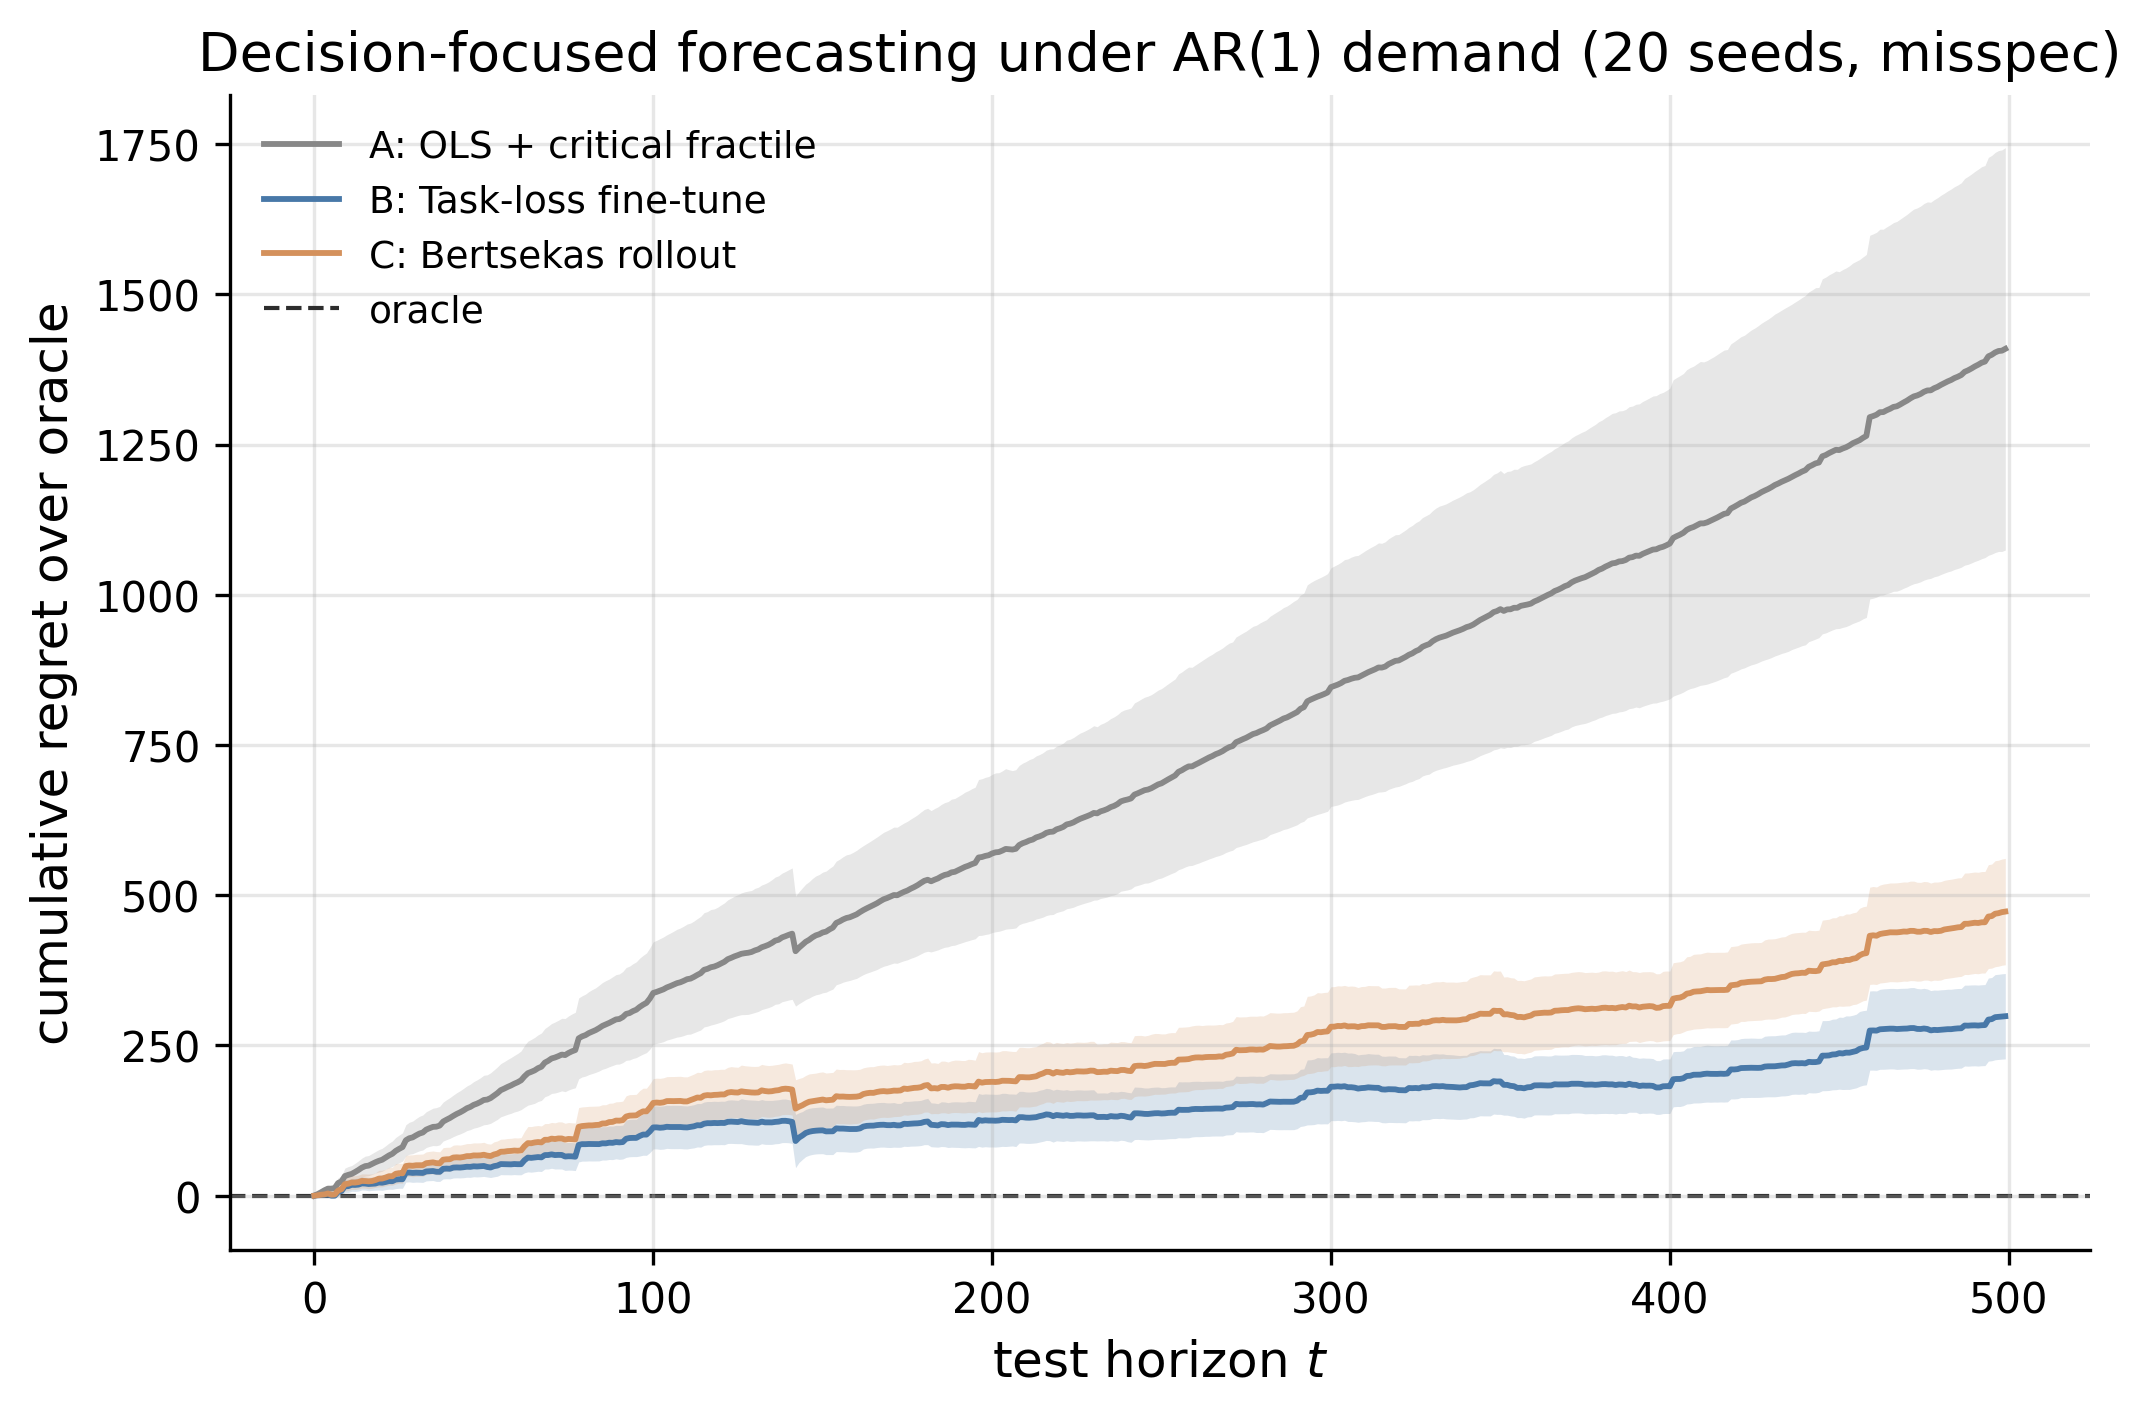
\includegraphics[width=0.85\linewidth]{../ch12_forecasting_rl/sims/decision_focused_ar1.png}
\caption{Cumulative newsvendor regret over the test horizon, $20$
seeds. The shaded band is one standard error of the mean. The
horizontal line at zero is the oracle. Method B (SPO$^+$ fine-tune)
attains the lowest regret; Method A (OLS plus critical fractile) the
highest.}
\label{fig:forecasting_rl_sim}
\end{figure}

Table~\ref{tab:forecasting_rl_sim} reports the realised costs. Method
A's in-sample MSE is $44.91 \pm 18.70$ and Method B's is $45.65 \pm
18.79$, statistically indistinguishable. Method C inherits Method A's
MSE by construction. The MSE ranking declares the three forecasters
equivalent. The realised newsvendor regret over $500$ test periods
diverges sharply. Method A attains $2.82 \pm 0.67$, Method B attains
$0.60 \pm 0.14$, and Method C attains $0.95 \pm 0.18$. Method B's
regret is a factor of $4.7$ lower than Method A's, and Method C's is a
factor of $3.0$ lower, both with standard errors that exclude zero.
Figure~\ref{fig:forecasting_rl_sim} plots the cumulative regret over
the test horizon.

The pattern is the Granger-Pesaran phenomenon of Section~\ref{sec:bridge}
on a familiar substrate. The MSE ranking and the decision-induced
ranking disagree once the noise model is misspecified, and a forecaster
that trades off in-sample squared error for in-sample realised cost
wins on realised cost out of sample. The simulation is also a worked
example of the \citet{HuKallus2020} counterpoint. Under
well-specification with $\gamma = 0$ the three methods are
indistinguishable on regret as well as on MSE, so the case for
decision-focused training and rollout is conditional on the
heteroscedasticity that the homoscedastic OLS model cannot represent.
The remainder of this section asks what changes when the decision is
sequential rather than one-shot.

\subsubsection{Sequential: approximate dynamic programming for forecasters}
\label{sec:adp}

The single-period newsvendor of \S\ref{sec:dfl} becomes a sequential
problem the moment the retailer carries inventory between periods. Today's
order $a_t$ affects tomorrow's starting state $s_{t+1}$, and the
realised cost $L(a_t, y_t)$ aggregates into a discounted return
$\sum_{t \ge 0} \gamma^t L(a_t, y_t)$. The standard dynamic programming
recursion gives the optimal policy via the Bellman equation
$V^\star(s) = \min_a \{ \mathbb E_y[L(a, y) + \gamma V^\star(s')]\}$, with
$s'$ the next state. The exact recursion is intractable whenever the
state space is high-dimensional or the next-state transition is unknown,
which is the regime that motivates approximate dynamic programming and
its modern reinforcement-learning descendants.

\citet{BertsekasRollout2022} provides the unifying frame for ADP applied
to sequential estimation. A measurement policy at time $k$ is a function
from the current posterior $b_k$ over an unknown parameter $\theta$ to
the next observation point $u_{k+1}$, and the exact dynamic programming
recursion
\begin{equation}
J^\star_k(b_k) = \min_{u_{k+1}}\Bigl\{
  c(u_{k+1}) + \mathbb E_{z_{u_{k+1}}}\bigl[
    J^\star_{k+1}\bigl(B_k(b_k, u_{k+1}, z_{u_{k+1}})\bigr)
  \bigr] \Bigr\}
\label{eq:bertsekas_dp}
\end{equation}
is infeasible because the posterior space is infinite-dimensional. The
rollout approximation replaces the unknown optimal continuation
$J^\star_{k+1}$ with the cost-to-go of a base policy
$\widetilde J_{k+1}$ that can be evaluated by Monte Carlo simulation. The
cost-improvement guarantee, namely that the rollout policy weakly
dominates the base policy under a mild contractivity condition, is the
formal underpinning of the entire programme. Certainty equivalence
further reduces the Monte Carlo burden by replacing the stochastic
continuation cost with its expectation conditional on the realised first
step. The same vocabulary covers Bayesian optimisation, sequential decoding,
and adaptive Bayesian experiment design.

\citet{Fernandes2024} applies the neuro-dynamic-programming variant of this
machinery to quarterly gross domestic product nowcasting. The Bellman
equation is
\begin{equation}
J(i) = \min_u \mathbb E\bigl[ g(i, u, j) + \alpha\, J(j) \bigr],
\label{eq:fernandes_bellman}
\end{equation}
where $i$ is the current state of the economy (regularised levels of
industrial production, construction output, retail trade turnover, goods
exports, goods imports, and the European Commission's Economic Sentiment
Indicator), $u$ is the quarter-over-quarter change of output, the cost
$g(i, u, j) = u^2$ is a quadratic adjustment cost in the spirit of
Lucas-Prescott (1971), and $\alpha \in (0, 1)$ is the discount factor. The
reward signal is not the cross-sectional forecast error of OLS. It is the
temporal difference between successive predictions of the GDP level. The
value function $J^\star$ is approximated by a single-hidden-layer
feed-forward network and trained by Sutton's temporal-difference algorithm.

\begin{algorithm}[h]
\caption{TD(0) with neural cost-to-go approximation \citep{Fernandes2024}}
\label{alg:fernandes_td0}
\begin{algorithmic}[1]
\State $\delta \gets \widetilde J(i, r) - \alpha \widetilde J(j, r) - g(i, u, j)$
\State $r_k \gets r_k - \gamma\, \delta\, h_k(i)$
  \Comment{output-layer update}
\State $r_{k\ell} \gets r_{k\ell} - \gamma\, \delta\, r_k\,
  \nabla_{r_{k\ell}} h_k(i)$
  \Comment{hidden-layer update}
\State \Return $r$
\end{algorithmic}
\end{algorithm}

Training uses a panel of $26$ European Union countries with $2{,}470$
quarterly transitions across $2000$Q1 to $2023$Q4, with Portugal held out
for evaluation over $2015$Q1 to $2023$Q4. Two findings matter for the
chapter. On the regularised Portuguese GDP level, the OLS benchmark
fitted on Portugal-only data attains a mean absolute error of $6.61\%$ of
the range and a root mean squared error of $8.32\%$. The TD-trained
neural network on the EU-ex-Portugal panel attains $4.53\%$ MAE and
$5.97\%$ RMSE, a $32\%$ reduction in MAE and a $28\%$ reduction in RMSE
relative to OLS. A linear architecture trained with the same TD algorithm
on the same panel attains only $10.70\%$ MAE, which establishes that the
gain is attributable to the nonlinear approximation and not to the
panel-data augmentation alone. The second finding is methodological. The
panel-data training transfers cleanly to the held-out country, which
alleviates the small-$T$ problem that plagues macroeconomic forecasting
and is the most concrete macro-domain validation of NDP on record.

A distinct strand uses reinforcement learning not as the forecaster
directly but as a meta-algorithm that adapts ensemble weights over a
portfolio of base forecasters \citep{Fu2022}. The state is the recent
window of the time series plus a log of per-model performance, the
action is a vector of non-negative weights on the simplex, and the
reward is the negative one-step forecast error. The methodological
contribution is modest. The model-combination problem is also an online
learning problem, and Hedge or EXP3 attains the same $O(\sqrt{T \log N})$
regret rate against the best fixed combination in hindsight. We mention
this strand for scope and move on.

\subsubsection{The boundary: deep inventory management}
\label{sec:madeka}

The sequential constructions of \S\ref{sec:adp} still produce a
forecaster as their artifact. Their most developed industrial instance is
the deep inventory-management system of \citet{Madeka2022DeepInventory},
who treat periodic-review inventory control with stochastic vendor lead
times, lost sales, correlated demand, and price matching as a sequential
decision problem whose forecast object is the joint distribution of
demand and lead time over a finite horizon. The technical device is
DirectBackprop, a differentiable historical-data simulator that lets
policy gradients flow through the realised inventory cost while the
exogenous processes are resampled from history. A learned ordering policy
parametrised by a deep network beats classical newsvendor and model-free
reinforcement-learning baselines on more than $10{,}000$ Amazon SKUs,
which makes it the direct multi-period generalisation of the
\citet{BanRudin2019} single-period empirical risk minimisation.

The reason this is the boundary of the RL-for-forecasting direction,
rather than a member of it, is a reduction theorem.
\citet{Madeka2022DeepInventory} prove that for the exogenous-decision-process
subclass, in which the dynamics depend on exogenous shocks but the agent's
actions do not feed back into demand or lead time, the
reinforcement-learning problem reduces to supervised learning against the
realised cost.\footnote{The reduction recovers the $\sqrt{p/n}$ regret
rate of \citet{BanRudin2019} as a special case and supplies a
finite-sample bound for the sequential version.} When that condition
holds, the sequential problem is decision-focused supervised learning
carried across a horizon, and the word reinforcement is ceremonial. When
the condition fails, that is, when the agent's actions move the
distribution of future demand or prices, the reduction breaks and the
problem is genuinely reinforcement learning. That distinction is the
hinge of the chapter. Sections~\ref{sec:model_based_planning}
and~\ref{sec:forecaster_as_policy} take up the regime on the far side of
it, where the forecaster is no longer the artifact but a component inside
the agent.

% Section 4: Forecasting for RL -- model-based planning (Story 2, part 1)
\subsection{Forecasting for RL: model-based planning}
\label{sec:model_based_planning}

Section~\ref{sec:rl_for_forecasting} kept the forecaster as the artifact.
This section and the next invert the relation. The forecaster becomes a
component inside a reinforcement-learning agent, and the artifact is a
policy. The boundary established in \S\ref{sec:madeka} marks the entry.
Once the agent's actions feed back into the data-generating process, the
reduction to supervised learning fails and the problem is genuinely
reinforcement learning.

The object the agent now needs is a forecaster of its own environment.
Given a state $s$ and an action $a$, it must predict the next state and
reward, $\widehat P(s', r \mid s, a)$. An economist will recognise this
object. Strip the action argument and it is the state-space model that
underlies the Kalman filter and the ARIMA family. Restore the action and
it is the controlled state-space model, the autoregressive system with
exogenous inputs that control engineers and macroeconometricians have
fitted for decades.\footnote{The state-space forecasting tradition is
surveyed in \citet{DurbinKoopman2012}. The controlled generalisation, in
which an exogenous input enters the transition equation, is standard in
both the control literature and the macroeconometric vector-autoregression
literature.} The recurrent state-space model at the core of the Dreamer
architecture below is the neural generalisation of exactly that object.
Two ingredients separate a world model from its classical ancestor. The
action enters the transition, and the model is trained against a value
functional rather than a likelihood. The first ingredient is structural.
The second is the sequential form of the bridge of
Section~\ref{sec:bridge}, and it is the subject of \S\ref{sec:vaml_ve}.
The empirical architectures that put the two ingredients together are the
subject of \S\ref{sec:world_models}.

\subsubsection{Value-aware model learning}
\label{sec:vaml_ve}

The bridge of Section~\ref{sec:bridge} has a sequential form. Estimating
the transition kernel $\widehat P$ by maximum likelihood treats every
component of the next-state distribution as equally informative. The
downstream planner cares about only one functional of it, namely
$(\widehat P V)(s, a) = \mathbb E_{s' \sim \widehat P(\cdot \mid s, a)}
[V(s')]$ for value functions $V$ in some candidate class. A value-aware
loss aligns the model-learning objective with that functional, in direct
analogy to the single-period decision-focused losses of \S\ref{sec:dfl}.

\citet{FarahmandVAML2017} formalise the alignment as the value-aware
model-learning (VAML) loss
\begin{equation}
\mathcal L_{\mathrm{VAML}}(\widehat P)
= \sup_{V \in \mathcal V} \bigl\| (\widehat P V) - (P^\star V) \bigr\|_\mu,
\label{eq:vaml_loss}
\end{equation}
where $\mathcal V$ is the candidate value class, $P^\star$ is the true
kernel, and $\| \cdot \|_\mu$ is an $L^2$ norm under a state-action
distribution $\mu$. They prove a finite-sample upper bound on the
value-suboptimality of the policy planned in $\widehat P$ that decomposes
into a model-approximation term, an estimation term that shrinks at the
parametric rate, and a complexity term in
$\mathcal V$.\footnote{An alternative regularity-restricted form is the
Wasserstein-VAML equivalence of \citet{AsadiWasserstein2018}. When
$\mathcal V$ is the class of $1$-Lipschitz value functions,
$\mathcal L_{\mathrm{VAML}}$ coincides with the $1$-Wasserstein distance
between $\widehat P(\cdot \mid s, a)$ and $P^\star(\cdot \mid s, a)$ by
Kantorovich-Rubinstein duality, which gives an optimal-transport reading
of value-aware learning.} \citet{FarahmandIterVAML2018} embeds
\eqref{eq:vaml_loss} inside approximate value iteration. At iteration $k$,
the model is fit to minimise the value-prediction error against the
current iterate $V_k$ rather than against the full class $\mathcal V$,
which turns the optimisation into a tractable regression and yields an
LSPI-style performance bound on the converged policy.

The full generalisation is \citet{GrimmVALEQ2020}'s value-equivalence
principle. Two models $\widehat P_1, \widehat P_2$ are value-equivalent
with respect to a policy set $\Pi$ and a value-function set $\mathcal V$
when $(T_{\widehat P_1}^\pi V)(s) = (T_{\widehat P_2}^\pi V)(s)$ for every
$\pi \in \Pi$ and $V \in \mathcal V$, where $T_{\widehat P}^\pi$ is the
Bellman operator under model $\widehat P$ and policy $\pi$. The
equivalence class shrinks monotonically as $\Pi$ and $\mathcal V$ grow,
collapsing to the singleton $\{P^\star\}$ in the limit of all policies and
all value functions. The principle subsumes Value Iteration Networks, the
Predictron, Value Prediction Networks, TreeQN, and the MuZero family of
\S\ref{sec:world_models} as instances that train a learned model against
narrow $(\Pi, \mathcal V)$ rather than against observation
likelihood.\footnote{\citet{GrimmPVE2021} sharpen the result for the
MuZero loss specifically. Their proper value equivalence relaxes the
equivalence relation to the $k$-step Bellman operator and bounds the
value suboptimality of the planned policy in terms of the model's loss on
a value-policy pair drawn from the planner. The bound formalises why
MuZero can plan well with models that fail at observation prediction.}

\citet{AyoubVTR2020} convert the value-aware idea into a regret
guarantee. In their value-targeted regression (VTR) algorithm, the model
at episode $k$ is fit by
\begin{equation}
\widehat P_k \in \arg\min_{P \in \mathcal P}
\sum_{t < k} \Bigl(
  (P V_t)(s_t, a_t) - V_t(s_{t+1})
\Bigr)^2,
\label{eq:vtr_loss}
\end{equation}
where $V_t$ is the most recent value-function iterate and $\mathcal P$ is
a linear-mixture model class. They prove a regret bound of
$\widetilde O\bigl(d \sqrt{H^3 T}\bigr)$, where $d$ is the model-class
dimension, $H$ is the horizon, and $T$ is the number of episodes. The
result is the first regret guarantee in which model fitting is driven by
a value-prediction loss rather than by a likelihood, and the rate matches
a known $\Omega(\sqrt{d H T})$ lower bound up to $H$ and logarithmic
factors. The value targets in \eqref{eq:vtr_loss} are themselves
policy-dependent and evolve through the learning loop, which is what
makes value-aware model learning irreducibly reinforcement learning
rather than the supervised special case of \S\ref{sec:madeka}.

Value-aware losses are not without pitfalls. \citet{VoelckerCalib2025}
show that the MuZero loss and several of its variants are uncalibrated in
the surrogate-loss sense of Section~\ref{sec:bridge}. The population
minimiser of the MuZero loss can be a transition kernel whose induced
value function differs from $V^\star$ even when $V^\star$ lies in the
function class. They propose a calibration correction that couples the
model class with a stochastic latent architecture and recovers the right
population minimiser. The result transfers the calibration question that
occupied Section~\ref{sec:bridge} into the sequential setting and ties the
value-aware programme back to the proper scoring-rule machinery.

\subsubsection{Dyna and the world-model line}
\label{sec:world_models}

The idea of using a learned forecaster to generate experience for a
planner is old. \citet{sutton1990} introduced the Dyna architecture as
an integrated loop of three operations executed at every time step.
The agent acted in the real environment and collected a transition. It
updated a learned dynamics model from that transition. It then drew
simulated transitions from the learned model and ran value-iteration
backups on those simulations between every pair of real-environment
steps. The classical Dyna-Q instance kept a tabular maximum-likelihood
estimate of the transition and reward functions and used the simulated
backups to amortise the cost of real interaction. Dyna's lasting
contribution was conceptual rather than algorithmic. It made explicit
that the data the agent collects through interaction can be amplified
by a forecaster of the environment, that the forecaster's update and
the planner's update can run in the same outer loop, and that the
forecaster need not be a maximum-likelihood estimate even though the
original Dyna-Q chose it to be one. The classical caveat applied
already in 1990 and applies to every descendant. When the model is
inaccurate, the simulated transitions inject bias into the value
function, and the planner amplifies rather than corrects the error.
The value-aware programme of \S\ref{sec:vaml_ve} is the direct response
to that caveat at the loss-function level.

What the modern world-model literature adds is that the forecaster, the
value function, and the planner are trained jointly against the same
planning-relevant targets, which is the empirical face of the
value-equivalence principle of \S\ref{sec:vaml_ve}. Three architectural
families anchor the literature.

\citet{Schrittwieser2020MuZero} introduce the MuZero algorithm. A
representation network embeds the observation into a latent state $h_0$.
A dynamics network unrolls latent transitions
$h_{k+1}, r_{k+1} = g(h_k, a_k)$. A prediction network outputs a value
$v(h_k)$ and a policy prior $\pi(h_k)$ at each unrolled step. The three
networks are trained jointly against three planning-relevant targets at
every unrolled depth $k$, namely the empirical Bellman target for $v$,
the bootstrapped policy prior for $\pi$, and the realised reward for $r$.
No observation-reconstruction loss is used. The latent dynamics network
is therefore a value-equivalent model in the sense of
\citet{GrimmVALEQ2020} rather than a generative forecaster of pixels.
Embedded inside Monte Carlo Tree Search, the resulting agent matches
AlphaZero on Go, chess, and shogi without access to game rules, and
attains state of the art on $57$ Atari games without a simulator.
\citet{Antonoglou2022StochMuZero} extend the algorithm to stochastic
environments by replacing the deterministic latent dynamics with
afterstate-plus-chance-node representations, with matching performance on
$2048$ and backgammon.

A complementary line of work uses an explicit probabilistic model of the
dynamics together with model-predictive control. \citet{Chua2018PETS}
introduce probabilistic ensembles with trajectory sampling. The dynamics
model is an ensemble of probabilistic neural networks that captures both
aleatoric uncertainty, through the per-network output variance, and
epistemic uncertainty, through ensemble disagreement. At each control
step, candidate action sequences are scored by Monte Carlo rollouts
through the ensemble and the first action of the best sequence is
executed. The model-predictive-control step is a one-step rollout in the
sense of \citet{BertsekasRollout2022}, and the ensemble is the
probabilistic forecast that feeds it. The combination attains the
asymptotic performance of model-free baselines such as soft actor-critic
and proximal policy optimisation while using between $8$ and $125$ times
fewer environment samples on standard continuous-control tasks, which is
the cleanest empirical case for probabilistic-dynamics-plus-rollout on a
benchmark suite that an econometrician would recognise.

The third family is the Dreamer line of recurrent state-space models.
\citet{HafnerDreamer2020} train a recurrent latent dynamics model from
pixels, plan in the compact latent space rather than in observation
space, and update the actor by backpropagating analytic value gradients
through imagined trajectories. DreamerV3 \citep{HafnerDreamerV3_2025}
scales the recipe across more than $150$ control tasks under a single
hyperparameter configuration and is the first algorithm to collect
diamonds in Minecraft from pixels and sparse rewards without human
demonstrations.\footnote{The Dreamer architecture keeps an
observation-reconstruction term in the world-model loss, which makes it
not strictly value-equivalent. The reconstruction loss regularises the
latent representation in ways that the MuZero-style pure value-target
objective does not. The \citet{VoelckerCalib2025} calibration analysis of
\S\ref{sec:vaml_ve} applies most directly to the MuZero family and remains
an open question for Dreamer-style models.}

These architectures still treat the forecaster as a component that feeds
a separate planner or value function. The next section turns to the more
radical inversion, in which the forecaster is the policy itself.

% Section 5: Forecasting for RL -- the forecaster as policy (Story 2, part 2)
\subsection{Forecasting for RL: the forecaster as policy}
\label{sec:forecaster_as_policy}
\label{sec:forecasting_in_rl}

Section~\ref{sec:model_based_planning} kept the forecaster as a component
that feeds a separate planner or value function. This section takes the
inversion further. The forecaster is the agent. Two flavours matter for
the chapter, namely trajectory generative models that treat the policy as
a forecast over future state-action sequences and counterfactual
forecasters that estimate the value of an alternative policy from logged
trajectories.

\subsubsection{Trajectory generative models}
\label{sec:trajectory_gen}

An offline reinforcement-learning dataset is a collection of trajectories
$\tau = (s_0, a_0, r_0, s_1, a_1, r_1, \dots, s_T, a_T, r_T)$ generated by
some behaviour policy. A trajectory generative model treats $\tau$ as a
sequence and trains a generative model on those sequences. The
\citet{Chen2021DT} Decision Transformer represents each trajectory as a
flat sequence
\begin{equation}
\tau = (\widehat R_0, s_0, a_0,\, \widehat R_1, s_1, a_1,\, \dots,\,
  \widehat R_T, s_T, a_T),
\label{eq:dt_sequence}
\end{equation}
where $\widehat R_t = \sum_{t' \ge t} r_{t'}$ is the return-to-go from
time $t$ onwards. A causally masked GPT-style transformer is trained to
predict the next action token given the last $K$ context tokens. At test
time, the operator specifies a desired return $R^\star$ and primes the
model with $\widehat R_0 = R^\star$ and the current state $s_0$. The model
generates the corresponding action, the environment returns a reward and
the next state, the operator decrements $R^\star$ by the realised reward,
and the loop repeats. No value function, no policy gradient, no critic
appears in training. The forecaster is the policy.

The empirical case rests on D4RL and Atari. On the $1\%$ DQN-replay slice
of Atari, the Decision Transformer attains gamer-normalised scores of
$267.5$ on Breakout against the $211.1$ of Conservative Q-Learning, the
incumbent offline-RL baseline. On the D4RL locomotion benchmark, the
Decision Transformer averages $74.7$ across nine task-dataset
combinations against CQL's $54.2$ and behavioural cloning's
$47.7$.\footnote{The same trajectory-as-sequence reframing was independently
proposed by \citet{Janner2021TT}, with beam search over tokenised states
and actions replacing return conditioning. Subsequent diffusion variants
\citep{Janner2022diffuser,Ajay2023} replace autoregressive generation with
iterative denoising of an entire trajectory and dispense with dynamic
programming entirely. The methodological move is the same. Plan by
sampling from a generative model of structured objects rather than by
maximising a learned value function.} For economists familiar with
structural estimation, the conceptual draw is that a forecast distribution
over trajectories doubles as the policy itself. The conditioning variable
plays the role of a behavioural target rather than a payoff.

\subsubsection{Counterfactual forecasting for off-policy evaluation}
\label{sec:counterfactual_ope}

Off-policy evaluation asks the question every applied economist asks at
some point. Given a logged dataset generated by a behaviour policy
$\pi_{\mathrm{obs}}$, what would the return have been under an alternative
policy $\widetilde\pi$? Importance sampling estimators are unbiased under
common support but high variance. Model-based estimators are low variance
but biased by model misspecification. The counterfactual route of
\citet{Buesing2019} sits between the two.

The construction casts the partially observable Markov decision process as
a structural causal model. The transition mechanism is
$s_{t+1} = f^s(s_t, a_t, u^s_t)$ with exogenous noise $u^s_t$, the
observation mechanism is $o_t = f^o(s_t, u^o_t)$, and the action
mechanism is $a_t = f^\pi(h_t, u^a_t)$ given the history. Given an
observed trajectory $\hat\tau$, the counterfactual rule has three steps.

\begin{algorithm}[h]
\caption{Counterfactual off-policy evaluation \citep{Buesing2019}}
\label{alg:buesing_cfope}
\begin{algorithmic}[1]
\State \emph{Abduction.} Infer the posterior $P(U \mid \hat\tau)$ over the
exogenous noise from the observed trajectory.
\State \emph{Action.} Replace the behaviour-policy mechanism $f^\pi$ with
the target-policy mechanism $f^{\widetilde\pi}$ to form the modified SCM
$\mathcal M^{\mathrm{do}(\widetilde\pi)}_{\hat\tau}$ with the same posterior
on $U$.
\State \emph{Prediction.} Sample $U \sim P(U \mid \hat\tau)$ and roll out
the modified SCM to obtain counterfactual trajectories $\tau^{\mathrm{cf}}$
and their returns.
\end{algorithmic}
\end{algorithm}

Lemma~1 of \citet{Buesing2019} establishes that the marginal of the
counterfactual distribution over $\hat\tau$ equals the interventional
distribution. The counterfactual estimator is unbiased under correct SCM
specification. On the partially-observable grid-world experiment of the
paper, the counterfactual estimator's evaluation error decreases
monotonically with the amount of off-policy data, while the model-based
estimator's error remains stuck at the bias of the dynamics model.

The categorical-action case raises an identification problem.
\citet{Oberst2019} show that multiple structural causal models can be
consistent with the same interventional distribution yet imply different
counterfactual outcomes, and resolve the ambiguity by assuming a
Gumbel-max sampling mechanism that satisfies a counterfactual-stability
condition.\footnote{The Pearl monotonicity condition resolves the binary
case. The Gumbel-max SCM is the natural extension to $k$-way categorical
outcomes. \citet{TangWiens2023} combine SCM-based counterfactual outcomes
with importance sampling to obtain variance reductions while preserving
unbiasedness under correct human annotation, with a sepsis-simulator
demonstration that delivers an RMSE of $0.013$ against $0.113$ for vanilla
per-decision IS.} The shared identifying assumption across this strand is
that the structural causal model is correctly specified. The Lucas
critique applies in its sharpest form when the agent's policy itself
enters the data-generating process. Identification by instruments or by
exogeneity restrictions, in the spirit of \citet{Chernozhukov2018}, is the
econometric remedy and remains an open research question for the
counterfactual-RL programme. The full econometric identification toolkit
for sequential confounded settings, namely backdoor adjustment,
instrumental variables, proximal and partially-observed bridges, and
mediator-based identification, is developed in the chapter on causal
inference for reinforcement learning; the structural-causal-model
machinery of this subsection is its structural complement rather than its
substitute.

\subsubsection{Simulation: counterfactual OPE under a misspecified SCM}
\label{sec:cfope_sim}

A second synthetic instance illustrates the counterfactual machinery on a
substrate that mirrors the contextual-bandit reading of
Section~\ref{sec:counterfactual_ope}. The DGP is a linear structural
causal model in two features,
\begin{equation}
y = 1 + 0.5\, x_1 - 0.3\, x_2 + 2\, a + a \cdot x_1 + u,
\qquad u \sim \mathcal N(0,\, 0.5^2),
\label{eq:cfope_dgp}
\end{equation}
with $x \sim \mathcal N(0, I_2)$, a binary action $a \in \{0, 1\}$, and
a heterogeneous treatment effect $\tau(x) = 2 + x_1$. The behaviour
policy $\pi_{\mathrm{obs}}(a = 1 \mid x) = \sigma(0.5 + x_1 - 0.5\, x_2)$
is confounded with $x$. The target policy $\widetilde\pi(a \mid x) =
\mathbf 1\{x_1 + x_2 > 0\}$ is a deterministic threshold rule. The
oracle value $V(\widetilde\pi) = \mathbb E_x[y \mid a =
\widetilde\pi(x)]$ is computed by Monte Carlo at $10^6$ realisations.

Three estimators are compared on $n \in \{200, 500, 1000, 2000\}$ logged
samples, $20$ seeds per cell. Per-decision importance sampling is
$\widehat V_{\mathrm{IS}} = n^{-1} \sum_i \rho_i y_i$ with $\rho_i =
\mathbf 1\{a_i = \widetilde\pi(x_i)\} / \pi_{\mathrm{obs}}(a_i \mid
x_i)$. The model-based plug-in $\widehat V_{\mathrm{MB}} = n^{-1}
\sum_i \hat f(x_i, \widetilde\pi(x_i))$ uses an OLS fit $\hat f$ on the
logged data. The counterfactual estimator follows the Buesing
abduction-action-prediction rule and combines $\hat f$ with a
residual correction weighted by the importance ratio,
\begin{equation}
\widehat V_{\mathrm{CF}}
= n^{-1} \sum_i \hat f(x_i, \widetilde\pi(x_i))
  + n^{-1} \sum_i \rho_i \bigl(y_i - \hat f(x_i, a_i)\bigr),
\label{eq:cfope_dr}
\end{equation}
which is the doubly-robust form of the abduction-action-prediction rule
and is unbiased under correct propensity \emph{or} correct
model.\footnote{The naive average of the per-observation counterfactual
outcome $y'_i = \hat f(x_i, \widetilde\pi(x_i)) + (y_i - \hat f(x_i,
a_i))$ collapses to $\widehat V_{\mathrm{MB}}$ under OLS with an
intercept, because the OLS residuals sum exactly to zero. The
importance-weighted residual correction in \eqref{eq:cfope_dr} restores
the bias-cancellation property in finite samples. The estimator
coincides with the classical doubly-robust estimator of
Robins-Rotnitzky-Zhao adapted to off-policy evaluation.} The
well-specified scenario uses the feature set $\{1, x_1, x_2, a,
a \cdot x_1\}$ in $\hat f$, matching the DGP. The misspecified scenario
drops the interaction $a \cdot x_1$, the source of the heterogeneous
treatment effect.

\begin{table}[h]
\centering
\caption{Counterfactual off-policy evaluation under a linear SCM,
$n = 1000$, $20$ seeds. The CF estimator's residual correction cancels
the MB bias under misspecification while inheriting low variance from
the model.}
\label{tab:cfope_summary}
% Generated by counterfactual_ope.py
\begin{tabular}{llccc}
\hline\hline
Scenario & Estimator & Bias & Std & RMSE \\
\hline
Well-specified & IS & $+0.017$ & $0.100$ & $0.099$ \\
 & MB & $-0.001$ & $0.057$ & $0.056$ \\
 & CF & $+0.003$ & $0.067$ & $0.065$ \\
\hline
Misspecified & IS & $+0.017$ & $0.100$ & $0.099$ \\
 & MB & $-0.072$ & $0.061$ & $0.093$ \\
 & CF & $+0.002$ & $0.078$ & $0.076$ \\
\hline\hline
\end{tabular}

\end{table}

\begin{figure}[h]
\centering
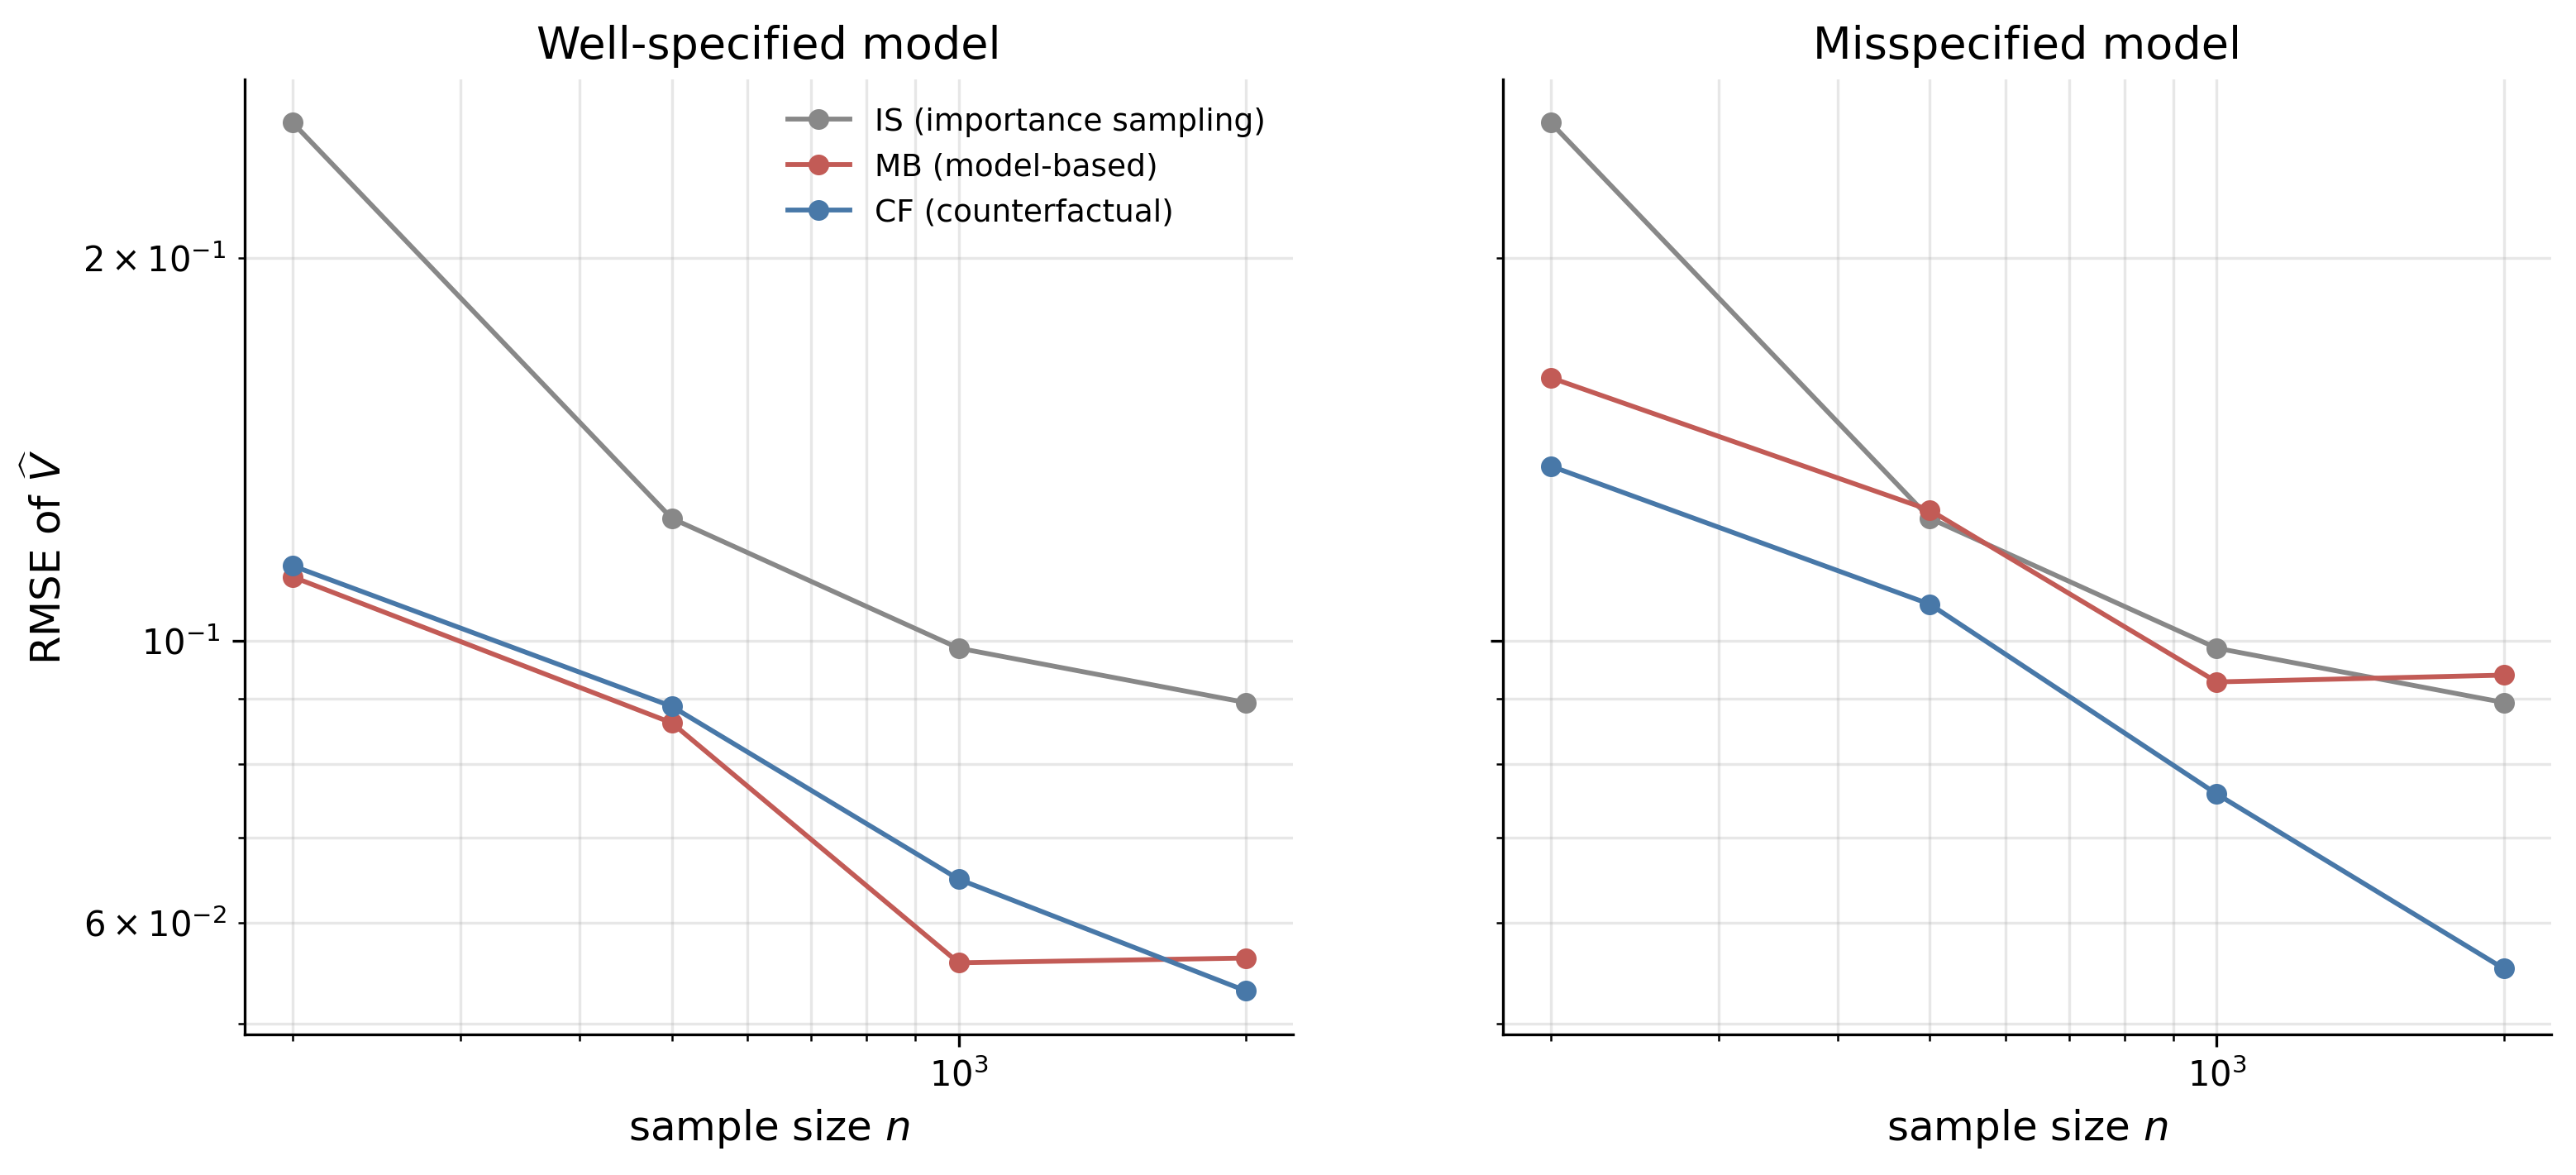
\includegraphics[width=0.85\linewidth]{../ch12_forecasting_rl/sims/counterfactual_ope.png}
\caption{Root mean squared error of three OPE estimators against the
sample size, log-log scale, two panels. Left panel: well-specified
outcome model. Right panel: misspecified model (interaction omitted).
The MB estimator's RMSE plateaus under misspecification as the bias
dominates the variance; the CF estimator's RMSE continues to decline.}
\label{fig:cfope_rmse}
\end{figure}

Table~\ref{tab:cfope_summary} reports bias, standard deviation, and
root mean squared error at $n = 1000$. Under well-specification, the
model-based estimator attains bias $-0.001$ and RMSE $0.056$, the
counterfactual estimator attains bias $0.003$ and RMSE $0.065$, and the
importance-sampling estimator attains bias $0.017$ and RMSE
$0.099$. The MB and CF estimators are statistically indistinguishable
and both improve on IS. Under misspecification, the MB estimator's
bias jumps to $-0.072$ and its RMSE to $0.093$, while the CF
estimator's bias remains at $0.002$ and its RMSE at $0.076$. The CF
estimator's RMSE is $18\%$ lower than MB's, and the bias is two orders
of magnitude smaller. The IS estimator is unchanged across scenarios
because it does not use an outcome model.
Figure~\ref{fig:cfope_rmse} plots RMSE against $n$ on log-log scale.
The MB curve flattens under misspecification at the population bias of
the OLS projection, the CF curve continues to decline at the parametric
rate, and the IS curve traces the higher-variance parametric rate that
the importance-weighted estimator delivers without any model
assistance.

The two simulations of the chapter make the same methodological point
on two different decision structures. The decision-focused AR(1)
forecaster of Section~\ref{sec:forecasting_rl_sim} beats the
prediction-focused OLS forecaster on realised newsvendor cost
precisely when the noise model is misspecified. The counterfactual OPE
estimator above beats the model-based estimator on RMSE precisely when
the outcome model is misspecified. The corrective in both cases is a
training or evaluation objective that knows about the decision-induced
loss, not the marginal forecast loss. The recipe extends naturally to
sequential and to non-stationary settings, where decision-focused
regret bounds at rate $T^{-1/4}$ exist under a margin condition on the
decision polytope \citep{Capitaine2025} and the extension to
action-conditional foundation forecasters remains a research frontier.

